% This section should describe the overall structure of your software system. Think of it as the strategy for how you will build the system. An architectural "layer" is the top-level logical view, or an abstraction, of your design. Layers should be composed of related elements of similar capabilities, and should be highly independent of other layers, but should have very clearly defined interfaces and interactions with other layers. Each layer should be identified individually and should be unique as to its function and purpose within the system. This section should also contain the high-level block diagram of the layers, as shown in the example below, as well as detailed descriptions of the functions of each layer.
The system for our product is currently simplified into 4 layers and 3 high-level components. Each layer/component will interact with one another in different ways.

\begin{figure}[h!]
	\centering
 	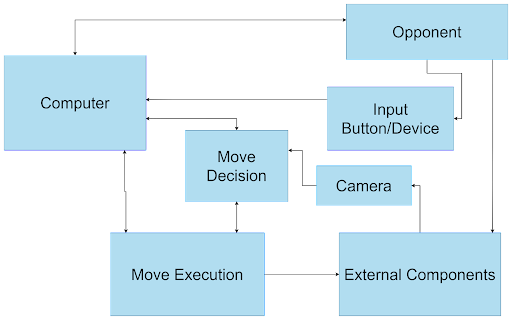
\includegraphics[width=0.60\textwidth]{images/layers}
 \caption{A simple architectural layer diagram}
\end{figure}

% \subsection{Layer X Description}
% Each layer should be described separately in detail. Descriptions should include the features, functions, critical interfaces and interactions of the layer. The description should clearly define the services that the layer provides. Also include any conventions that your team will use in describing the structure: naming conventions for layers, subsystems, modules, and data flows; interface specifications; how layers and subsystems are defined; etc.

\subsection{Opponent Description}
The Opponent is the person that will be going against the robot during the checkers game. The opponent will interface with the Input Button/Device component, Computer layer, and External Components layer in order to progress and play checkers with the robot arm and make game moves.

\subsection{Input Button/Device Description}
The Input Button/Device is one of the ways the opponent will be able to facilitate the progression of the checkers match. When this component is pressed, it will notify the Computer layer that the human opponent has finished making their move.

\subsection{Camera Description}
The camera is the component that acts as the eyes into the real world for our system. The camera acts as a bridge that sends the AI layer the necessary information that it needs about the current state of the checkers board.


\subsection{Move Decision Layer Description}
The Move Decision layer is the layer that will make all of the move decisions that the robot will make. This layer consists of Computer Vision and AI. After receiving data about the current state of the board from the Camera, the Move Decision layer will formulate a move decision that will be sent to the Computer layer.

\subsection{Computer Layer Description}
The Computer layer is the central piece of our system. This layer contains the HUD, GUI, and Software components of our system. This layer acts as the facilitator of the checkers match, and receives input from the Opponent to progress the match, sends signals to the AI layer to grab board state and make a move, and signals the UR5 Robot Arm layer to execute those moves.

\subsection{Move Execution Layer Description}
The Move Execution layer is the layer that will physically execute the moves that our system will make during a checkers match. This layer consists of the Magnetic Gripper, the Arduino, and the UR5 Robot Arm. After receiving move data from the Computer layer, the Move Execution layer will interface with the components in the External Components layer to make its next move.

\subsection{External Components Layer Description}
The External Components layer is composed of all of the physical checkers board game pieces. Both the Opponent component and the Move Execution layer physically interact with the External Components layer when they have made their move decisions to progress the match. This layer is made up of the Playing Board, the Collection Box, and the Checkers Pieces.